\chapter{Developing an experimental setup for measuring the performance and
    near-wake of cross-flow turbines at large laboratory
    scale}\label{chap:exp-setup}

In 2011, a turbine test bed was developed for measuring the performance
(mechanical power and overall rotor drag or thrust) of large laboratory scale
($O(1)$ m\textsuperscript{2} frontal area) cross-flow turbines in the University
of New Hampshire (UNH) tow tank \cite{Bachant2011-MS}, a 36.6 m long, 3.66 m
wide, and 2.44 m deep facility, pictured in Figure~\ref{fig:tow-tank}, that was
capable of towing up to approximately 1.4 m/s. The turbine-specific
instrumentation consisted of a mounting frame built from NACA 0020 hydrofoil
struts, a hydraulic disk brake for turbine loading, an Interface T8 200 Nm
capacity rotary torque transducer, and a 54 pulse-per-rev magnetic pickup for
measuring shaft speed. The frame was mounted to the carriage via
streamwise-oriented linear bearings and was held in place by a pair of Sentran
ZB3 500 lbf load cells, to measure the overall streamwise rotor drag.

\begin{figure}[ht]
    \centering
    
    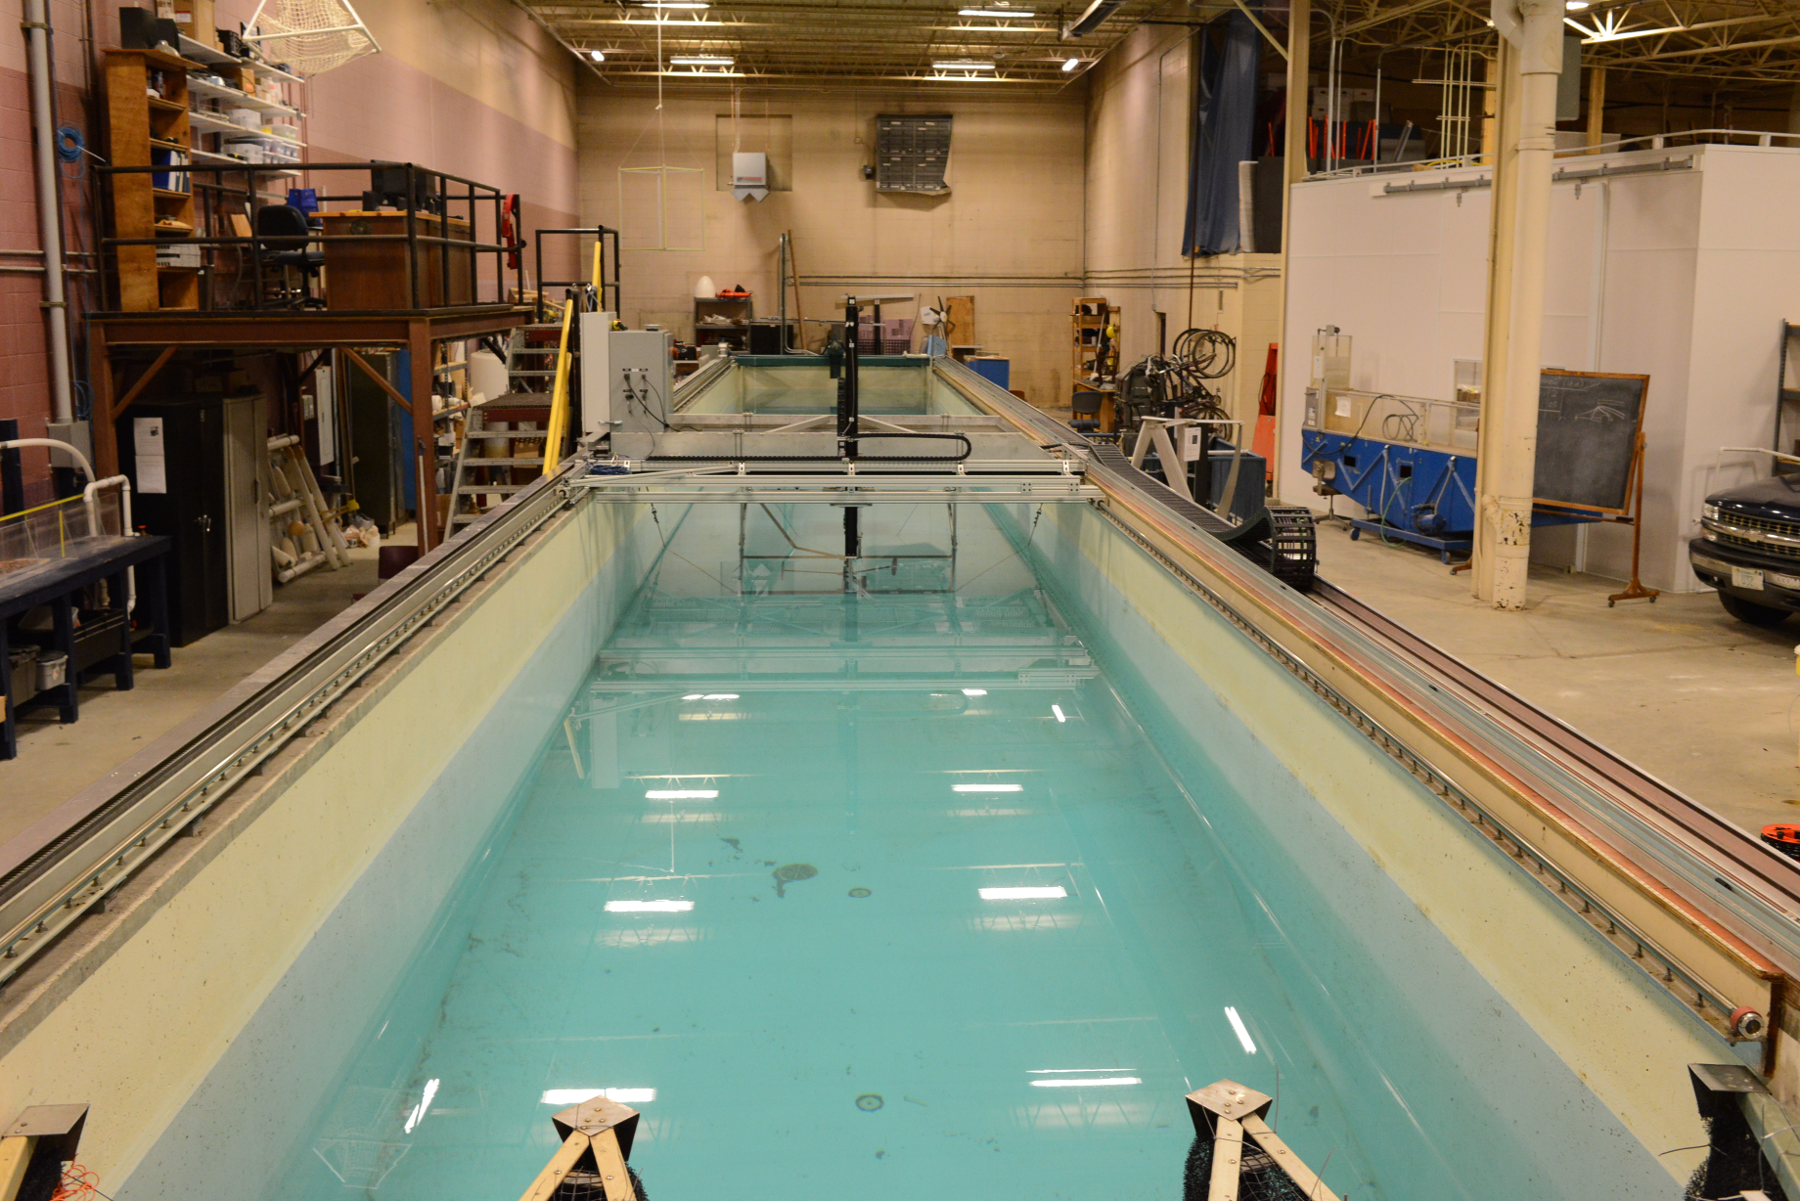
\includegraphics[width=0.9\textwidth]{tow-tank.png}
    
    \caption{The University of New Hampshire's wave and tow tank, located in the
        Jere A. Chase Ocean Engineering Laboratory.}
    
    \label{fig:tow-tank}
\end{figure}

Despite its usefulness in producing a relatively small amount of data for two
helical cross-flow turbines~\cite{Bachant2015-RE}, the existing system had some
issues to be addressed:
\begin{itemize}
    \item No control over turbine shaft angular velocity. This made operation at
    tip speed ratio below peak torque impossible.
    
    \item Fully manual starting and load application. This limited resolution of
    the applied torque, and took considerable effort to perform experiments on
    the order of 100 tows, since a person had to ride on the carriage to adjust
    and apply the load torque.
    
    \item Open loop speed and manual position control of the tow carriage. This
    also took considerable effort to operate experiments, since the operator had
    to estimate braking distance to ensure the carriage did not hit the tank
    ends.
    
    \item Low carriage acceleration. The carriage acceleration was on the order
    of 0.1 m/s\textsuperscript{2}, which limited the steady state turbine
    operating duration to a few seconds.
    
    \item Low frequency resonance in the tow member. A long 0.25 inch diameter
    wire rope was used to tow the carriage, which resonated longitudinally with
    the significant variation of streamwise forces from the turbine.
\end{itemize}

In addition to the above issues, in order to meet the data acquisition goals, it
was necessary to measure turbine wake flows. These concerns required major
renovations, upgrades, and additions to the tow tank and turbine test bed
motion, control, and data acquisition systems. Furthermore, it was desirable to
automate the entire system to increase both data quality and quantity. These
changes were made possible thanks to an infrastructure grant from the US
Department of Energy (DOE).


\section{Modifications to the UNH tow tank}

The ``foundation'' of the experimental setup was the tow tank, which was
addressed first. The main goals for the tow tank upgrades were to increase max
speed and acceleration, add closed-loop positioning and velocity control,
stiffen the tow member to reduce longitudinal resonance, and add onboard power
and networking to the carriage for data acquisition and other peripherals. A
summary of the old system and new target specifications is shown in
Table~\ref{tab:tow-tank-specs}.

\begin{table}
\centering
\begin{tabular}{c|c|c}
Spec & Old system & Target \\ 
\hline
Maximum speed & 1.4 m/s  & 3.0 m/s \\ 
Maximum acceleration & 0.1 m/s$^2$ & 2.0 m/s$^2$ \\ 
Control system & Open loop velocity only & Closed loop position/velocity \\ 
Onboard power & $4\times12$ V batteries & Continuous 120 and 220 VAC \\ 
\end{tabular}
\caption{Specifications summary for existing and upgraded tow tank systems.} 
\label{tab:tow-tank-specs}
\end{table}


\subsection{Linear guides}

The previous linear guide system consisted of a ``master'' guide constructed
from $4 \times 4$ inch fiberglass tubing, and a ``slave'' guide constructed from
aluminum angle, on which plastic wheels rode. Over time, the fiberglass tubing
had failed structurally and was covered with stainless steel bars fixed with
double-sided tape. These bars shifted around considerably during towing and were
a source of noise.

A new set of linear guides was designed from 1.25 inch diameter Thomson 440C
stainless steel linear shafts and super self-aligning linear bearings. The
existing carriage was modified to retrofit the linear bearings, and a series of
parts were designed to adapt the stainless shafts to the existing quasi-level
mounting surfaces, which helped keep cost down. The shafts were mounted via
3/8-24 inch threaded rods in oversized holes to allow adjustment in all three
dimensions, a concept which was inspired by similar linear guide setups at the
University of Minnesota's Saint Anthony Falls Laboratory (SAFL). The shafts were
aligned in the cross-tank direction using a piece of monofilament line stretched
along the path. The vertical alignment was set by spacing the shaft from its
mounting surface equally along the path via machined blocks. When the existing
level surfaces were set in 1996, these were measured to be level within $\pm
1/16$ inches~\cite{Darnell1996}.


\subsection{Motion and control}

The tow tank's previous motion system consisted of a 10 horsepower AC induction
motor powered by a Yaskawa V7 variable frequency drive. The motor was coupled to
a speed reducing gearbox, on which a pulley was mounted to drive a 0.25 inch
diameter wire rope. It was seen in previous testing that this system had very
low acceleration ($\sim 0.1$ m/s$^2$), which severely reduced steady state
towing durations. The relatively low spring constant of the wire rope tow member
also gave the system a low natural frequency, which resonated due to cross-flow
turbines' cyclic forcing. Furthermore, the system was only velocity-controlled,
and in an open-loop manner. This meant positioning was done manually, which took
a skilled operator, and reduced usable tank length further to allow for coasting
to a stop.

These issues were addressed by changing the motor to a Kollmorgen AKM82
permanent magnet servo motor and 10:1 gearbox, sized to tow turbines with 1
m$^2$ frontal area up to 3 m/s, while accelerating at 2 m/s$^2$. The motor was
powered by a Kollmorgen S700 servo drive, controlled by an 8-axis ACS NTM
EtherCAT master controller, providing closed loop position and velocity control.
A series of emergency stop buttons were also installed to increase the safety of
the system.

A 7.5 cm wide steel-reinforced polyurethane timing belt was chosen as the new
drive member. The most robust timing belt profile---an ATL20---was chosen for
maximum stiffness per unit width. Custom timing belt and pulley housings were
designed to move both the upper and lower runs of the belt above the tank wall,
shortening the overall length, which when combined with the higher specific
stiffness belt increased the total drive member spring constant roughly by a
factor of 7.


%%% From RM2 test plan %%%


\begin{figure}[ht!]
    \centering 
%    \includegraphics[clip,trim=0 0.4in 0 0.37in, 
%    width=0.49\textwidth]{Figures/tow_tank_length} 
%    \includegraphics[clip,trim=0.67in 0 0 0, 
%    width=0.49\textwidth]{Figures/test_bed_photo} 
    \caption{Photos of the UNH towing tank and turbine test bed.} 
%    \label{fig:tow-tank}
\end{figure}


\begin{table}[ht]
    \centering
    \begin{tabular}{c|c|c|c}
        Measured quantity & Device type & Mfg. \& model & Nominal accuracy \\
        \hline 
        Carriage position & Linear encoder & Renishaw LM15 & 10 $\mu$m/pulse \cite{RenishawLM15}\\
        Turbine angle & Servo encoder output & Kollmorgen AKD & 10$^5$ pulse/rev \cite{KollmorgenAKD}\\
        Turbine torque & Rotary transducer & Interface T8-200 & $\pm$0.5 Nm \cite{InterfaceT8}\\ 
        Turbine torque (2) & Load cell (\& arm) & Sentran ZB3-200 & $\pm$0.2 Nm \cite{SentranZB}\\
        Drag force, left & Load cell & Sentran ZB3-500 & $\pm$0.6 N \cite{SentranZB}\\
        Drag force, right & Load cell & Sentran ZB3-500 & $\pm$0.6 N \cite{SentranZB}\\
        Fluid velocity & ADV & Nortek Vectrino+ & $\pm$0.5\% $\pm$1 mm/s \cite{NortekVectrino}\\
    \end{tabular}
    \caption{Details of the sensors to be used for the experiment. Note that ``(2)''
        denotes a secondary redundant measurement. ``Turbine torque (2)'' nominal
        accuracy estimated by combining load cell accuracy and arm machining tolerances
        ($\pm 1 \times 10^{-4}$ m) as root-sum-square.} \label{tab:sensors}
\end{table}

\begin{table}[ht]
    \centering
    \begin{tabular}{c|c|c}
        Measured quantity & Device type & Mfg. \& model \\
        \hline 
        Carriage position & Differential counter & NI 9411 \\
        Carriage velocity (2) & Motion controller & ACS NTM \\
        Turbine angle & Differential counter & NI 9411 \\
        Turbine RPM (2) & Motion controller & ACS NTM \\
        Turbine torque & Analog voltage input & NI 9205 \\ 
        Turbine torque (2) & Analog bridge input & NI 9237 \\
        Drag force, left & Analog bridge input & NI 9237 \\
        Drag force, right & Analog bridge input & NI 9237 \\
    \end{tabular}
    \caption{Details of the instrumentation to be used for the experiment. Note that
        ``(2)'' denotes a secondary redundant measurement.}
    \label{tab:instrumentation}
\end{table}

\begin{figure}[ht]
    \centering
%    \includegraphics[clip,trim=0.01in 0 0 0, width=0.95\textwidth]{Figures/tank_cross_section}
    \caption{Illustration of the experimental setup.}
    \label{fig:exp-setup}
\end{figure}


\begin{figure}[ht]
    \centering
    %\begin{subfigure}[t]{\textwidth}
    %    \centering
    %    \includegraphics[width=0.7\textwidth]{figures/exp-setup-photo}
    %    \caption{}
    %    \label{fig:exp-setup-photo}
    %\end{subfigure}
    
    %\begin{subfigure}[t]{\textwidth}
    %    \centering
    %    \includegraphics[width=0.7\textwidth]{figures/exp_setup_drawing}
    %    \captiton{}
    %    \label{fig:exp-setup-dwg}
    %\end{subfigure}
    
    \caption{Experimental setup photo (a) and drawing (b): turbine test bed
        installed in the UNH tow tank.}
    
    \label{fig:exp-setup}
\end{figure}


%%% End section from RM2


\subsection{Data acquisition and onboard accessories}

The previous generation tow tank data acquisition (DAQ) system was based around
an onboard PC, powered by a set of four 12 V automotive batteries. This was
done to avoid the complexity of running power out to the carriage
\cite{Darnell1996}. The DAQ PC was accessed via Windows Remote Desktop to
control any DAQ applications. The PC that sent the control signal to the
inverter drive was a separate machine, which meant users had to work with at
least two interfaces to specify DAQ and motion parameters. This also made it
difficult to synchronize motion with data acquisition, e.g., triggering data
collection at a certain location.

A new DAQ system was designed based around a National Instruments (NI) 9188
CompactDAQ Ethernet chassis. NI 9237, 9205, 9401, and 9411 modules were
installed for analog bridge, analog voltage, digital, and quadrature encoder
signals, respectively. A single CAT5e cable was dedicated for this system.
Additional cables were run for the EtherCAT and Internet connectivity on the
carriage. An 8-port Ethernet-serial server was installed for accessing serial
devices, e.g., the Nortek Vectrino+, described later. For measuring carriage
speed, and therefore inflow velocity, a Renishaw LM15 linear encoder with 10
$\mu$m resolution was installed and connected to the NI 9411 module. Networking,
power, and control signal cables were run through an igus cable carrier,
installed along the ``slave'' or $+y$ side of the tank.

Requirements for onboard power were derived from the goal of fully automating
both motion and data acquisition. It was also determined that the UNH ME
department's high frame rate particle image velocimetry (HFR-PIV) system would
be used on the carriage at some point, which included laser power supplies and a
laser chiller that could not be powered by the previous generation's isolated
battery/inverter system. 

An onboard electronics cabinet was designed by Minarik, inc. as part of the
upgraded motion system. A 45 amp, 120 VAC circuit and 20 amp, 240 VAC single
phase power cable were run through the cable carrier to power outlets on the
side of the onboard electronics cabinet. An additional 240 VAC three-phase
supply was connected to a Kollmorgen AKD servo drive, also installed in the
cabinet, which was sized to power a servo motor to control turbine shaft
position and speed. The AKD drive's digital outputs were setup for triggering
instrumentation, e.g., the NI 9188 chassis, via the main motion controller.


\section{Upgraded turbine test bed}

For this work, the turbine test bed was kept mostly intact, but modified for
fully-automated operation. To reduce low frequency resonance in the frame caused
by turbine side forces, and help redistribute some of the streamwise force from
turbines towed at higher speeds, two pairs of steel guy wires were added. These
solutions were chosen based on a finite element analysis (FEA) of the turbine
mounting frame, which showed more improvement regarding stiffening in the
desired directions compared to simply adding 45 degree flat bar braces in the
corner joints. To ensure drag from the outer guy wires was included in the
overall streamwise force measurement, an additional set of linear bearings was
added to the carriage for their connection.


\subsection{Turbine loading, speed control, and torque measurement}

In order to control turbine shaft angular velocity, a Kollmorgen AKM62Q servo
motor and 20:1 ratio gearhead were added with a custom retrofit mounting plate
and housing. Two zero-backlash R+W EKH/300/B curved jaw couplings were added
above and below the rotary torque transducer. An additional torque measurement
system was added by mounting the servo/gearhead assembly to a slewing ring
bearing, and holding its mounting housing in place by a Sentran ZB3 200 lbf load
cell attached at a fixed distance by a 16 inch long arm. This system served as a
redundant torque measurement for values up to 200 Nm, and extended the maximum
torque range to approximately 360 Nm.

Turbine shaft speed was measured via the AKD drive's emulated encoder output,
set to $5 \times 10^3$ (pre-gearbox) or $1 \times 10^5$ (post-gearbox)
lines-per-rev in an A-quad-B configuration. This signal was sampled by either
the NI 9401 (Chapter~\ref{chap:RVAT-baseline}) or the NI 9411
(Chapters~\ref{chap:Re-dep} and \ref{chap:RM2}) modules.


%%% From RVAT-Re-dep

Experiments were performed in a turbine test bed specifically designed for
cross-flow turbines. The test bed was integrated as part of the University of
New Hampshire (UNH) tow tank, which is a 36 m-long facility with a 3.66 m-wide
and 2.44 m-deep cross-section. The turbine model used in this study was the UNH
Reference Vertical Axis Turbine (RVAT), which was designed to be a generic case
for numerical model testing, similar to the Sandia National Labs/U.S. Department
of Energy Reference Model 2 (RM2) River Turbine \cite{Neary2014}, but with a
higher solidity or blade chord-to-radius ratio.

The turbine was mounted in a frame constructed from NACA 0020 sections, shown in
Figure~\ref{fig:exp-setup}. The turbine shaft ran up through the water surface,
coupled to a Kollmorgen AKM permanent magnet servo motor (Kollmorgen, Radford,
VA, USA) with a 20:1 gearbox, providing precise control over shaft angular
velocity. This servo was controlled by the tow tank's main motion controller for
high synchronization with the carriage motion, thereby giving precise
measurement and control of the tip speed ratio. An Interface T8 200 Nm capacity
rotary torque transducer (Interface, Scottsdale, AZ, USA) was installed inline
between the servo and the turbine, and the servo was also mounted on a slewing
ring bearing, which allowed a redundant measurement of torque via an arm and
load cell used to counteract the turbine moment. The frame was mounted to the
carriage via linear guides, such that the total streamwise drag force was
transferred to a pair of Sentran ZB3 500 pound-force capacity S-beam load cells
(Sentran, Santa Ana, CA, USA), providing the rotor drag measurements, after a
separately measured tare drag was subtracted in post-processing. Similarly, a
tare torque was measured by rotating the turbine shaft in air. Turbine angular
and tow carriage linear position were measured using quadrature encoder signals,
with $10^5$ counts-per-rev for the turbine and 10 ${\mu}$m resolution for the
carriage position. These~signals, along with the torque and drag signals, were
sampled at 2 kHz.

Wake velocity was measured using a Nortek Vectrino+ acoustic Doppler velocimeter
(ADV) (Nortek AS, Rud, Norway), which has an approximately 6~mm diameter
sampling volume and sampled at 200 Hz. The probe was mounted on an automated
positioning system, also controlled by the tow tank's main motion controller.
The ADV and data acquisition systems' sampling times were synchronized by
triggering the start of data acquisition via a pulse sent from the motion
controller. Additional details of the turbine and experimental setup are
described in \cite{Bachant2015-JoT}.

%%% End from RVAT-Re-dep


\subsection{Wake measurement system}

In order to characterize turbine wakes, a Nortek Vectrino+ acoustic Doppler
velocimeter (ADV) was purchased as part of the upgraded tow tank
instrumentation. An ADV is capable of measuring three components of velocity at
a single point in space, and the Vectrino+ can sample at 200 Hz. This system is
considered desirable compared with hot wire or hot film anemometry as there are
no calibrations, and the sensor element is significantly more robust. Spatial
resolution is typically lower---on the order of 1 cm \cite{NortekVectrino}---but
this is still small compared with the typical length scale of a turbine model.
ADV is also preferable to laser Doppler velocimetry (LDV) in this case since the
tow carriage is a high vibration environment, which would make LDV alignment a
challenge.

A $y$--$z$ axis positioning system was designed for the Vectrino probe. This
system consisted of two Velmex BiSlide linear stages---the $y$-axis driven by
belt and the $z$ by ball screw. Both drive systems were powered by stepper
motors with approximately 0.001 inch resolution. These motors were driven by an
ACS UDMlc EtherCAT drive, connected to the tow tank's main motion controller for
integrated synchronous motion.

When operating the Vectrino, the tank was seeded with 11 micron mean diameter
hollow glass spheres. Seeding was added along the tank length, generally at the
surface, and was mixed by towing the turbine through the tank. This process was
repeated until the Vectrino's signal-to-noise ratio (SNR) was approximately
above 12 dB. Note that while acquiring ADV data the $y$- and $z$-axis stepper
drive had to be disabled to reduce noise. The axes were re-enabled to position
the probe before each run.


\subsection{Software}

Software was developed to automate the entire turbine testing process. Dubbed
\textit{TurbineDAQ}, the desktop application was written in Python due to its
reputation as a good ``glue'' language for systems integration. The graphical
user interface (GUI) was built using the PyQt bindings to the Qt framework.
Communication with the tow tank's motion controller, data acquisition system,
and ADV were integrated into a single application. This combined with the
ability to load and automatically execute test matrices in comma-separated value
(CSV) format allowed for experiments consisting of thousands of tows, where the
previous generation could only realistically achieve around 100.


\subsection{Tare drag and torque compensation} 

The drag and torque measurement systems were set up in such a way that raw
measurements for drag would include all submerged gear and torque would include
all friction below the transducer along with the turbine shaft torque. To
compensate, tare torque and drag runs were to be performed to measure the shaft
bearing friction torque and turbine mounting frame drag, respectively. These
data will be similar to the turbine performance data, omitting torque
measurements for the tare drag runs and vice versa. Tare drag runs will be
performed for each tow speed in the experiment, for which the mean value is used
in data processing. Tare torque runs will be performed by rotating the turbine
shaft (without blades) in air at constant angular velocity for a specified
duration, over the range of angular velocities used throughout the experiment.
Tare torque will then be fit with a linear regression versus shaft angular
velocity, and added to the measured turbine torque in post-processing.


\subsection{Synchronization of instrumentation subsystems}

The three data acquisition instrumentation subsystems---motion controller, NI
DAQ (performance measurements), and Vectrino+ (wake velocity
measurements)---were set to begin sampling at precisely the same time each run,
after being triggered by a TTL pulse created by the motion controller. This
strategy retains synchronization for all performance signal samples (tow speed,
torque, drag, angular velocity), ensuring precise calculation of, e.g., power
coefficient. Since there is also synchronization of the initial sample from each
three subsystems, correlation of events in the performance and wake signals is
also possible.


\subsection{Calibrations}

Factory calibrations for all instrumentation were used for the experiments
described in Chapters~\ref{chap:RVAT-baseline} and \ref{chap:Re-dep}. The drag
slide and torque arm assemblies were calibrated out of the tank using the
fixtures shown in Figure~\ref{fig:calibration-fixtures}, in which a Sentran ZB3
500 lbf capacity load cell and indicator were used for input values. The
reference load cell and indicator were calibrated as a full system from the
factory and remained connected to each other at all times. The drag slide and
torque arm fixtures were loaded incrementally using a 3/4-16 inch threaded rod,
nut, and self-lubricating thrust bearing.

\begin{figure}
    \caption{Torque arm and drag slide calibration fixtures.}
    
    \label{fig:calibration-fixtures}
\end{figure}

Before the RM2 experiment described later in Chapter~\ref{chap:RM2}, traceable
calibration certificates were obtained for the Interface T8-200 torque
transducer and NI 9205 and NI 9237 modules. In 2014, the drag slide and torque
arm assemblies were recalibrated using the same fixture and Sentran ZB3 load
cell and indicator described above, for which a new traceable calibration
certificate was obtained. Values before and after the recalibration are
presented in Table~\ref{tab:calibrations}.

\begin{table}
    \centering
\begin{tabular}{c|c|c|c}
    Signal & Calibration 1 & Calibration 2 & Difference \\ 
    \hline 
    Torque trans. & 40.0000 Nm/V & 39.8380 Nm/V & -0.4 \% \\ 
    Torque arm & 122531 Nm/V/V & 123437 Nm/V/V & 0.7 \% \\ 
    Drag left & 743104 N/V/V & 742830 N/V/V & -0.1 \% \\ 
    Drag right & 740137 N/V/V & 742400 N/V/V & 0.3 \% \\ 
\end{tabular}
    \caption{Calibration slopes used for experimental measurements. Calibration
        1 was used in Chapter~\ref{chap:RVAT-baseline} and
        Chapter~\ref{chap:Re-dep}. Calibration 2 was used in
        Chapter~\ref{chap:RM2}.}
    
    \label{tab:calibrations}
\end{table}


\section{Determining tank settling time}

Each experiment, sample tows were at each speed to determine the amount of time
taken between runs such that the tank has settled adequately, i.e., background
turbulence and any large scale mean flows have been dissipated. This was
assessed by towing the turbine, then allowing the Vectrino to continue recording
velocity data, monitoring the mean and standard deviation of the signals. The
settling times were then included in the experiment configuration---one value
for each tow speed, to be used by \textit{TurbineDAQ} as wait times between
automated runs.

\todo[inline]{Plot sample settling data.}


\section{Experimental uncertainty}

\todo[inline]{Vary the wording of uncertainty section a bit more.}

For each set of experimental measurements, it was imperative to estimate
uncertainty. Both systematic and random errors were considered. Random error was
inferred from the sample standard deviation (on a per-rotor-revolution basis)
and the systematic error was estimated from the sensor calibrations or
datasheets. Combination of both error sources and their propagation into derived
quantities, which is described below, followed those by Coleman and Steele
\cite{ColemanSteele}.

An expanded uncertainty interval with 95\% confidence was computed for mean
power coefficient $C_P$, mean rotor drag coefficient $C_D$, and mean wake
velocities
\begin{equation}
    U_{95} = t_{95} u_c,
\end{equation}
where $t_{95}$ is the value from the Student $t$-distribution for a 95\%
confidence interval and $u_c$ is the combined standard uncertainty, which is
given by
\begin{equation}
    u_X^2 = s_{\bar{X}}^2 + b_X^2,
\end{equation}
where $s_{\bar{X}}$ is the sample standard deviation of the mean per turbine
revolution. The systematic uncertainty $b_X$ is computed as
\begin{equation}
    b_{X}^2 = \sum_{i=1}^J \left( \frac{\partial X}{\partial x_i} \right)^2
    b_{x_i}^2,
\end{equation}
where $x_i$ is a primitive quantity used to calculate $X$ (e.g., $T$, $\omega$,
and $U_\infty$ for calculating $C_P$), and $b_{x_i}$ is the primitive quantity's
systematic uncertainty, estimated as half the value listed on the sensor
manufacturer's documentation.

Selecting $t_{95}$ requires an estimate for the number of degrees of freedom
$\nu_X$, which was obtained using the Welch--Satterthwaite formula:
\begin{equation}
    \nu_X = \frac{\left(s_X^2 + \sum_{k=1}^M b_k^2 \right)^2} {s_X^4/\nu_{s_X} +
    \sum_{k=1}^M b_k^4/\nu_{b_k}},
\end{equation}
where $\nu_{s_X}$ is the number of degrees of freedom associated with $s_X$ and
$\nu_{b_k}$ is the number of degrees of freedom associated with $b_k$.
$\nu_{s_X}$ is assumed to be $(N-1)$, where $N$ is the number of independent
samples (or turbine revolutions). $\nu_{b_k}$ was estimated as
\begin{equation}
    \nu_{b_k} = \frac{1}{2} \left( \frac{\Delta b_k}{b_k} \right)^{-2},
\end{equation}
where the quantity in parentheses is the relative uncertainty of $b_k$, assumed
to be 0.25.


\section{Blockage}

Putting a turbine in a confined environment such as a towing tank will force
flow through the turbine at higher velocity compared with a free case, where
streamlines are allowed to diverge. Consequently, higher levels of blockage will
lead to increased turbine performance, and a shift in optimal operating
parameters, i.e., tip speed ratio. In order to for experiments to be relevant to
others in the literature, blockage effects must either be corrected for, or the
blockage ratio should be kept to a typical value seen in other studies.

Most numerical models have the ability to include finite domains or walls, which
makes results even in blocked case applicable to validation. Furthermore,
blockage will be non-zero in most MHK cases, where turbines are placed in rivers
or channels, the effects of which need to be predicted as well.


\section{Turbine models}

Two physical turbine models were designed and built. The first was intended to
be a geometrically simple---i.e. symmetrical foil profiles, square frontal area,
rectangular blade planform---high-solidity turbine. This turbine was constructed
from materials donated by Lucid Energy Technologies, LLP, and dubbed the
``Reference Vertical-Axis Turbine'' or UNH-RVAT.

The second turbine was designed and built as part of a measurement task for
Sandia National Laboratories (SNL), in collaboration with the US Department of
Energy (DOE). The so-called ``Reference Model 2'' (RM2) was developed by SNL to
be a standard cross-flow turbine for which modelers could validate their
predictions \cite{Neary2014}. The RM2 was designed using Sandia's CACTUS vortex
line code \cite{Barone2011}, and its low solidity made it a nice complement to
the UNH-RVAT for testing the robustness of numerical models to varying solidity.


\subsection{UNH-RVAT}

A primary goal for the UNH-RVAT was geometric simplicity, for the sake of
replication in numerical models. The turbine was model constructed from straight
14 cm chord length NACA 0020 extrusions, used for both the blades and struts.
Blades were mounted at mid-chord, mid-span, and zero preset pitch, with a length
or height of 1 m and placed at 1 m diameter, giving the rotor an aspect ratio of
unity. These parameters gave the rotor a relatively high solidity $Nc/(\pi D) =
0.13$ and a large chord-to-radius ratio $c/R = 0.28$. 

The support struts were also constructed from 14 cm chord NACA 0020 profiles,
and attach the turbine to a 9.5 cm diameter shaft. A sketch of the turbine rotor
is shown in Figure~\ref{fig:unh-rvat} and CAD models are available from
\cite{Bachant2014-RVAT-CAD}.

\todo[inline]{Add drawing of UNH-RVAT.}
\begin{figure}[ht]
    \caption{Drawing of the UNH-RVAT vertical-axis cross-flow turbine. Note that
        the upper and lower mounting flanges have been excluded. These were included
        in the tare drag measurements for the experiments in
        Chapter~\ref{chap:Re-dep}, but excluded for those in
        Chapter~\ref{chap:RVAT-baseline}.}
    
    \label{fig:unh-rvat}
\end{figure}


\subsection{DOE/SNL RM2}

The RM2 rotor was designed as a 1:6 scale model of that described in the RM2
``rev 0'' design report \cite{Barone2011}, with the exception of the shaft
diameter, which was scaled from the SAFL RM2 shaft \cite{Hill2014}. The hub
design is also similar to the SAFL model. Geometric parameters are shown in
Table~\ref{tab:turb-geom} and a drawing of the turbine design is shown in
Figure~\ref{fig:RM2-drawing}. The turbine model components---blades, struts,
shaft, and center hub sections---were fabricated from 6061-T6 aluminum, which
was hardcoat anodized per MIL-8625-A, type III, class 2 specifications.

\begin{table}[ht]
    \centering
    \begin{tabular}{l|l|l}
        & Full-scale & Model (1:6) \\
        \hline 
        Diameter (m)   & 6.450 & 1.075 \\ 
        Height (m)     & 4.840 & 0.8067 \\ 
        Blade root chord (m) & 0.4000 & 0.06667 \\ 
        Blade tip chord (m)  & 0.2400 & 0.04000 \\ 
        Blade profile & NACA 0021 & NACA 0021 \\ 
        Blade mount & 1/2 chord & 1/2 chord \\ 
        Blade pitch (deg.) & 0.0 & 0.0 \\ 
        Strut profile & NACA 0021 & NACA 0021 \\ 
        Strut chord (m) & 0.3600 & 0.06000 \\ 
        Shaft diameter (m) & 0.2540 \cite{Beam2011} or 0.4160 \cite{Hill2014} & 0.06350\\ 
    \end{tabular}
    \caption{RM2 turbine geometric parameters.}
    \label{tab:turb-geom}
\end{table}

\begin{figure}[ht]
    \centering
%    \includegraphics[width=0.5\textwidth]{figures/rm2}
    \caption{Illustration of the 1:6 RM2 scaled physical model.}
    \label{fig:RM2-drawing}
\end{figure}


\section{Summary and conclusions}

An upgraded test bed for large laboratory scale ($O(1)$ m) cross-flow turbines
was developed for the UNH tow tank. To acquire adequate amounts of data and to
achieve significant lengths of steady state operation with a limited tank
length, the tow tank's linear motion, control, and data acquisition systems had
to be redesigned, rebuilt, and upgraded to allow fully automated operation,
along with higher carriage speed and acceleration.

The upgraded test bed increased the number of tows possible per experiment by
essentially an order of magnitude.

Two turbine models were designed and fabricated. The UNH-RVAT turbine was
designed to be more geometrically simple, but higher solidity, while the RM2
turbine is lower solidity, with tapered blades. The differences between these
rotors provide an opportunity for direct comparison within the same experimental
setup, and will provide validation data to test models' predictive capabilities
with varying levels of flow curvature (from higher $c/R$) and end effects (blade
aspect ratio and taper).
